\subsection{Rács elrendezés}

\begin{frame}
    Rács elrendezés
    \begin{itemize}
        \item Egy rács (grid) celláiba lehet elhelyezni a tartalmi elemeket. 
        \item Rács: szülő elem, cellák: beágyazott elemek.
        \item A cellák sorokba (row) és oszlopokba (column) rendeződnek. Oldalaikat képzeletbeli függőleges és vízszintes vonalak szegélyezik, melyek számozása 1-től, a bal felső sarokból kezdődik.
        \item A cellák között rések (gap) lehetnek.
    \end{itemize}
\end{frame}

\begin{frame}
    Rács tulajdonságai
    \footnotesize
    \begin{description}[m]
        \item[display] \hfill \\ Az elem tárolóvá alakítása, értékek: \texttt{grid} vagy \texttt{inline-grid}
        \item[grid-template-columns] \hfill \\ Oszlopok számának és méretének megadása, pl. \texttt{100px auto} két oszlopot eredményez. Az első 100 képpont széles, a maradékot a második oszlop foglalja el.
        \item[grid-template-rows] \hfill \\ Hasonlóan adja meg a sorokat.
        \item[row-gap] \hfill \\ Sorok közötti rés mérete.
        \item[column-gap] \hfill \\ Oszlopok közötti rés mérete.
        \item[gap] \hfill \\ Rövidítés, egy lépésben megadható \texttt{row-gap} és \texttt{column-gap} értéke. Egy érték esetén mindkettőt ugyanarra állítja be.   
    \end{description}
\end{frame}

\begin{frame}
    \begin{center}
        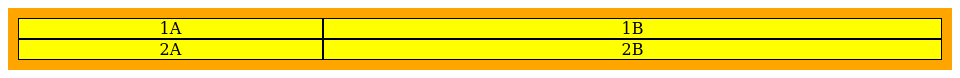
\includegraphics[width=\textwidth]{racs1.png} \\
    \end{center}
    \begin{columns}[T]
        \column{.4\textwidth}
            \begin{exampleblock}{\textattachfile{racs1.html}{HTML}}
                \vspace{-.3cm}
                \scriptsize
                \lstinputlisting[style=HTML,linerange={22-27},numbers=left,firstnumber=22]{racs1.html}
                \vspace{-.3cm}
            \end{exampleblock}
        \column{.55\textwidth}
            \begin{exampleblock}{\textattachfile{racs1.html}{CSS}}
                \vspace{-.3cm}
                \scriptsize
                \lstinputlisting[style=HTML,linerange={7-18},numbers=right,firstnumber=7]{racs1.html}
                \vspace{-.3cm}
            \end{exampleblock}
    \end{columns}
\end{frame}

\begin{frame}
    Rács igazítása (ha a tárolt elemek kisebbek a rendelkezésre álló helynél)
    \begin{description}[m]
        \item[justify-content] \hfill \\ Vízszintes igazítás
        \item[align-content] \hfill \\ Függőleges igazítás
    \end{description}
    \vfill
    Lehetséges értékek:
    \begin{columns}[T]
        \column{.25\textwidth}
            \begin{description}[m]
                \item[start] \hfill \\ Felülre / balra 
                \item[center] \hfill \\ Középre
                \item[end] \hfill \\ Alulra / jobbra
            \end{description}
        \column{.65\textwidth}
            \begin{description}[m]
                \item[space-around] \hfill \\ Két oldalon azonos méretű helyet hagy.
                \item[space-between] \hfill \\ A cellák között azonos méretű helyet hagy. 
                \item[space-evenly] \hfill \\ A cellák körül és köztük is azonos méretű helyet hagy. 
            \end{description}
    \end{columns}
\end{frame}

\begin{frame}
    \begin{center}
        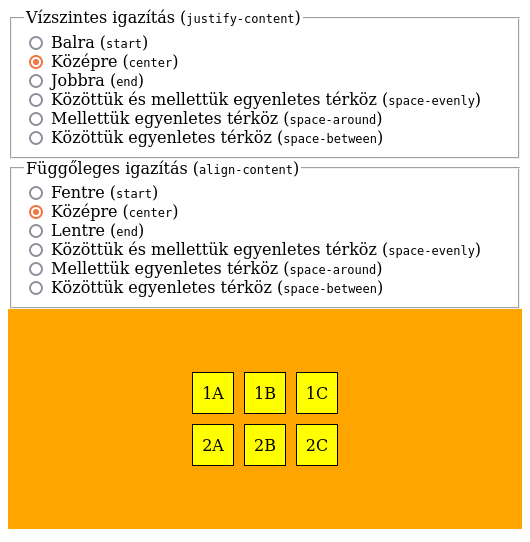
\includegraphics[scale=.3]{racs2.png} \\
        \textattachfile{racs2.html}{racs2.html}
    \end{center}
\end{frame}

\begin{frame}
    Cellák helye és méretei
    \begin{description}[m]
        \item[grid-column-start] \hfill \\ Melyik vonal után kezdődjön az elem? 
        \item[grid-column-end] \hfill \\ Melyik vonal előtt fejeződjön be? 
        \item[grid-column] \hfill \\ Előző két érték megadása egyben, pl. \texttt{1 / 5}. A záró vonal száma helyett megadható szélesség, pl. \texttt{1 / span 4}.
        \item[grid-row-start, grid-row-end, grid-row] \hfill \\ Ugyanez a sorokra vonatkozóan.
        \item[grid-area] \hfill \\ Bal felső sarok sora, oszlopa, majd jobb alsó sarok sora és oszlopa egy lépésben megadható, pl. \texttt{1 / 2 / 5 / 6}, vagy megadható a méret \texttt{span}-nal. 
    \end{description}
\end{frame}

\begin{frame}
    \begin{center}
        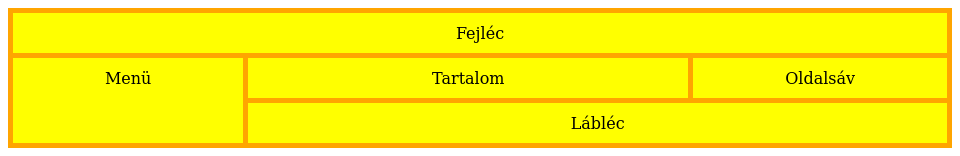
\includegraphics[scale=0.3]{racs3.png}
    \end{center}
    \begin{exampleblock}{\textattachfile{racs3.html}{HTML}}
        \footnotesize
        \lstinputlisting[style=HTML,linerange={41-47},numbers=left,firstnumber=41]{racs3.html}
    \end{exampleblock}
\end{frame}

\begin{frame}
    \begin{columns}
        \column{.5\textwidth}
            \begin{exampleblock}{\textattachfile{racs3.html}{CSS}}
                \scriptsize
                \vspace{-.2cm}
                \lstinputlisting[style=HTML,linerange={21-37},numbers=left,firstnumber=21]{racs3.html}
                \vspace{-.2cm}
            \end{exampleblock}
        \column{.4\textwidth}
            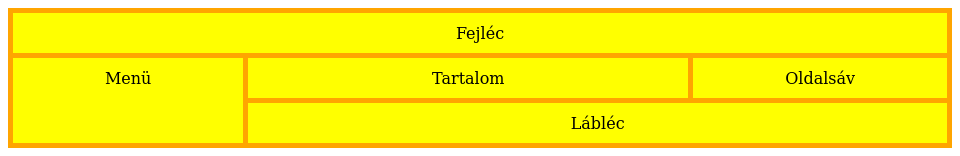
\includegraphics[width=\columnwidth]{racs3.png}
    \end{columns}
\end{frame}

\begin{frame}
    Hely és méret megadásának alternatív módja:
    \begin{itemize}
        \item Egyedi nevek megadása a tetszőleges méretű területekhez (\texttt{grid-area}).
        \item Táblázat minden cellájába beírjuk a terület nevét, ami lefedi azt (\texttt{grid-template-areas}).
    \end{itemize}
    \begin{exampleblock}{\textattachfile{racs4.html}{CSS}}
        \scriptsize
        \vspace{-.2cm}
        \lstinputlisting[style=HTML,linerange={7-16},numbers=left,firstnumber=7]{racs4.html}
        \vspace{-.2cm}
    \end{exampleblock}
\end{frame}

\begin{frame}
    \begin{exampleblock}{\textattachfile{racs4.html}{CSS}}
        \lstinputlisting[style=HTML,linerange={24-28},numbers=left,firstnumber=24]{racs4.html}
    \end{exampleblock}
\end{frame}